Storing high-dimensional vector data cannot be done efficiently with traditional databases. Vector databases (VDBs) specialize in efficiently searching for semantically similar entities within high-dimensional data. Especially for dense retrieval, similarity search is a highly complex topic. Given a query vector $v_1$, finding the nearest neighbor $v_{n}$ would require comparing $v_1$ with every vector in the dataset. Jing \cite{Jing.2024} notes this brute-force approach yields $O(dN+N$ $log$ $k)$ complexity, making it impractical for large-scale applications. Efficient alternatives to brute-force search constitute the key differentiating capability of modern vector database systems. To date, no comprehensive comparison of search latency across VDB providers exists to our knowledge. Pan \cite{Pan.2024} compared providers regarding features they offer and pointed out that cross-disciplinary comparisons of vector search algorithms and systems are scarce.

While numerous optimization techniques exist, this thesis focuses on two representative methods: We detail Product Quantization (PQ) and the Hierarchical Navigable Small World (HNSW) algorithm, a state-of-the-art approximate nearest neighbor (ANN) method—due to their widespread adoption and effectiveness. I refer to Jing \cite{Jing.2024} and Kukreja \cite{Kukreja.2023}, who explained many other techniques in great detail.

\paragraph{Hierarchical Navigable Small World (HNSW)}

\begin{figure}[h!]
    \centering
    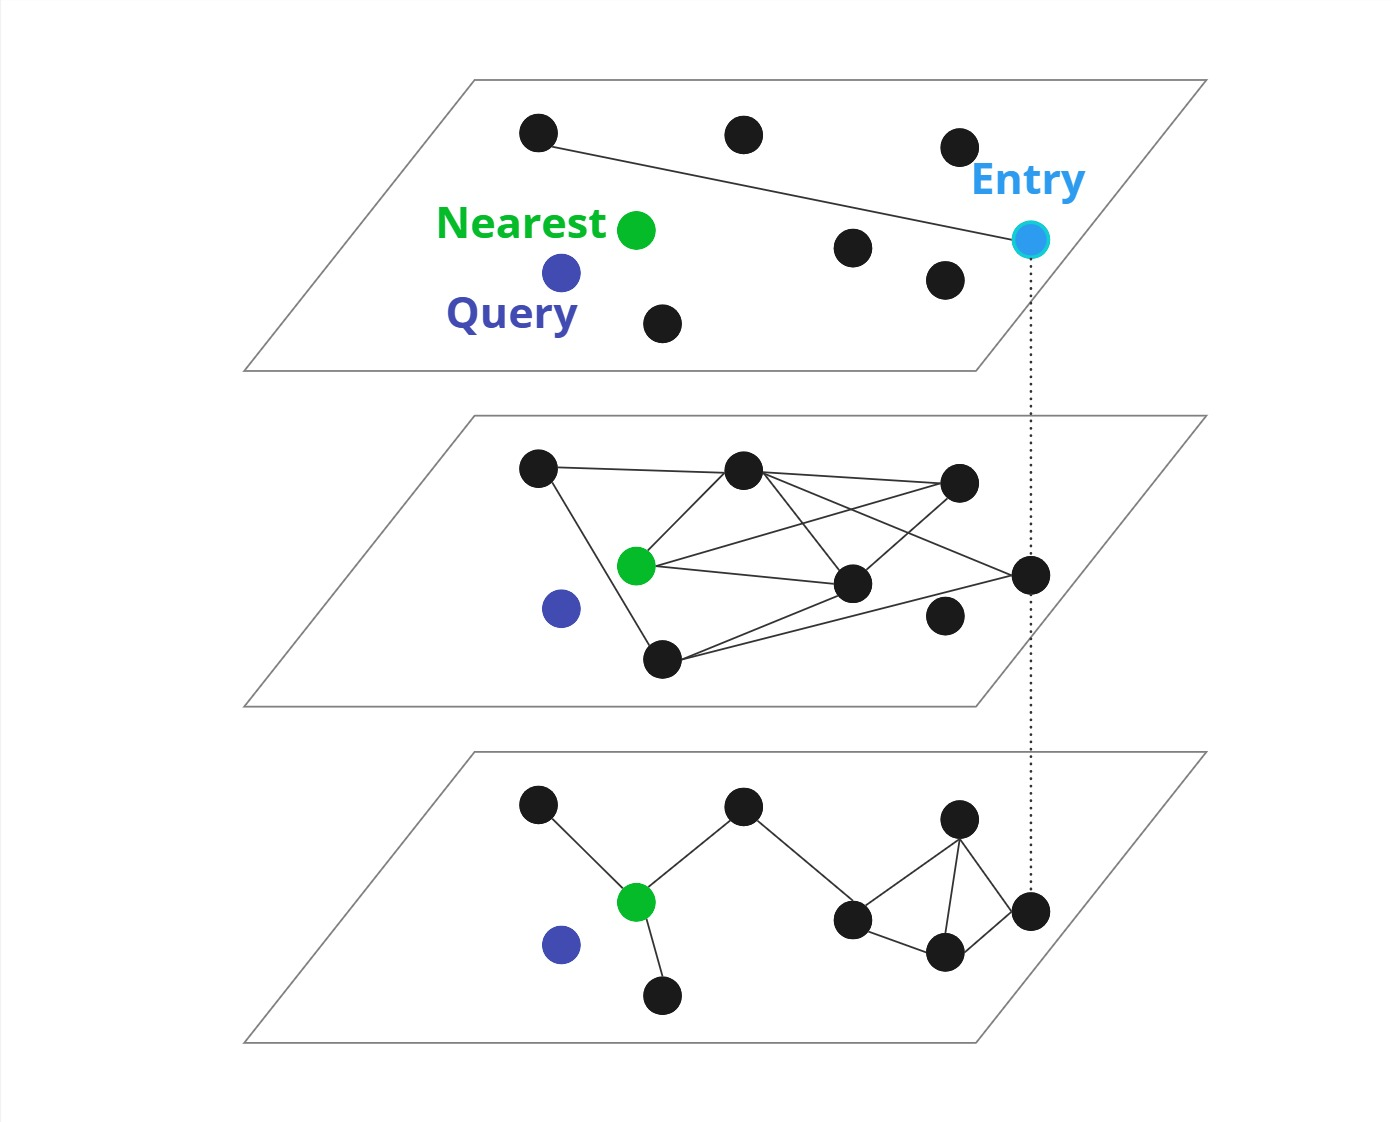
\includegraphics[width=\textwidth]{images/HNSW.jpg}
    \caption{HNSW algorithm visualized, highly inspired by \cite{Pinecone.22.01.2025}}
    \label{fig:HNSW}
\end{figure}

Approximate Nearest Neighbor is a term referencing all Nearest Neighbor algorithms that do not search for the most similar or closest point, but rather for a match that is close enough. One version of that is the HNSW algorithm, which was developed by \cite{Malkov.2014} and uses a skip-pattern invented by \cite{Pugh.1990}. The algorithm is visualized in figure \ref{fig:HNSW}. HNSW constructs a hierarchical graph where nodes connect via randomly sampled edges across multiple layers. Upper layers contain long-range connections, while lower layers progressively feature shorter, localized edges. The algorithm starts comparing on the top-level layer and if it reaches a local minimum, it continues on the next layer until it finds its local minimum on the bottom layer. While HNSW sacrifices guaranteed optimality, it achieves a favorable trade-off between recall and execution speed, as demonstrated by \cite{ErikBernhardsson.22.01.2025}.
